\documentclass[conference]{IEEEtran}
\IEEEoverridecommandlockouts
% The preceding line is only needed to identify funding in the first footnote. If that is unneeded, please comment it out.
\usepackage{cite}
\usepackage{amsmath,amssymb,amsfonts}
\usepackage{algorithmic}
\usepackage{graphicx}
\usepackage{textcomp}
\usepackage{xcolor}
\usepackage{kotex}
\usepackage{wrapfig}
\usepackage{makecell}
\usepackage{tabularx}
\usepackage{float}
\usepackage{supertabular,booktabs}
\def\BibTeX{{\rm B\kern-.05em{\sc i\kern-.025em b}\kern-.08em
    T\kern-.1667em\lower.7ex\hbox{E}\kern-.125emX}}
\begin{document}

\title{Golden Child \\
  {\LARGE The Communication Channel for Children and Parents} \\
  {\footnotesize \large Golden Child}
   }

\author{\IEEEauthorblockN{Kim Seohyun 2020028259}
\IEEEauthorblockA{\textit{College of engineering} \\
\textit{Hanyang University}\\
Seoul, Korea \\
hyununseo@gmail.com}
\and
\IEEEauthorblockN{Kim Hyunji 2020088222}
\IEEEauthorblockA{\textit{College of engineering} \\
\textit{Hanyang University}\\
Seoul, Korea \\
hyunjikim1218@gmail.com}
\and
\IEEEauthorblockN{Park Jiwon 2020020255}
\IEEEauthorblockA{\textit{College of engineering} \\
\textit{Hanyang University}\\
Seoul, Korea \\
park@jiwon.me}
\and
\IEEEauthorblockN{Lee Subin 2020000819}
\IEEEauthorblockA{\textit{College of engineering} \\
\textit{Hanyang University}\\
Seoul, Korea \\
supiao0123@gmail.com}
}

\maketitle

\begin{abstract}
  Today, conflicts with children are often intensified especially after puberty due to lack of conversation and communication between parents and children. The child wants to talk to the parents, but the parents are busy or have no time to face each other, so they gradually stop talking, and as this process is repeated, the conversation becomes difficult and the conversations dried up. In addition, parents need professional coaching to properly raise their children because they do not know what their children do in their daily lives.As on-tact communication, which means meeting online, is now common, we planned this project to help parents communicate with their children through our applications, pay attention to their thoughts and feelings and receive coaching of proper parenting.\\
\end{abstract}

\begin{IEEEkeywords}
Application, AI Speaker, Sentiment Analysis , NLP , Communication Channel, Child Rearing
\end{IEEEkeywords}


\newpage
{\large{Role Assignment}}
{\renewcommand{\arraystretch}{1.5}%
\begin{table}[h!]
\begin{tabular}{ | p{0.11\textwidth} | p{0.09\textwidth} | p{0.21\textwidth} | }
\cline{1-3} 
\textbf{Role} & \textbf{\textit{Name}}& \textbf{\textit{Task Description}}\\
\hline
User/Customer&All&Main user and customer of our application will be the parent and child. Therefore, we should be well known about parent, and especially child. User and customer have to think about arrangement of pages and accessibility of features in order to create a positive user experience. \\
\hline
Backend developer&Kim Hyunji Lee Subin&Backend developers think about backend systems which are needed in developing projects like using databases with SQL queries. We manage the server-side and database related to the process of a website, web application or mobile solution. As a backend developer, as many languages are provided like python, Java, Node.js, JavaScript.\\
\hline
Frontend developer&Kim Seohyun Park Jiwon&Frontend developers design UI/UX for applications to create the environments for users. Frontend developers should implement the design of the application considering user convenience. The ability to use React-Native, typescript, and css is needed.\\
\hline
Development manager&All&Development manager’s main role is to look at the software from various perspectives and control the entire process of software development. In particular, it is important for development manager to take advantage of their customers and give feedback to software developers. In addition, development managers should understand the market situation and consider the essential services that customers need.\\
\hline
\end{tabular}
\end{table}}
\newpage


\section{\large{Introduction}}

\subsection{\large{Motivation}}

We focused on the psychology of adolescents before forming their identity and created this ON-Tact conversation application that solves the disconnection of family conversation and forms an attachment between parents and children. In the past, family usually had a conversation during their meals when they gathered. However, as the number of double income family increases today, the time for family members to eat together is decreasing. And it is increasingly difficult to even see each other due to frequent overtime work. Since children also go to several academies, the time family members spend together is less than before. In addition to the lack of family time, there are many factors that interfere with family conversations such as watching TV or using smartphones, even if families are gathered at home. Parents and children become harder and harder to understand each other, and the conversation becomes disconnected. Therefore, the function of the home gradually faded from the space that gives stability and rest to the space where just sleeping and eating. In fact, a recent survey of teenagers showed that the average of conversation time between their family members was only about 13 minutes a day. It also showed the reason why children do not talk is that parents have a lack of empathy and understanding of them. Therefore, it is most important to share daily life and develop understanding in order to solve the disconnection of family conversation. According to a research paper, this process is especially important in the lower grades of elementary school when a child enters school. This period is also meaningful for children because it is a time when they grow out of their infancy and enter the school which allows them to start a social life. Parents are most interested in their children's school adaptation problems and academic problems during this period. The lower grades of elementary school are the most direct and honest parent-child conversation takes place. It is necessary to form a bond of sympathy at this time so that a desirable relationship with the parent-child can be maintained even when the child goes through puberty. This application can help parents-children communicate better with children who develop identity before puberty. First, when a parent registers question based on children's daily lives, children answer the question and share their daily life. Parents better understand the child's situation through these answers and communicate with the child by asking additional questions based on previous answer. The child realizes that his parents have great interest and affection for him through parents' questions. Since these interactions are not restricted in time and space, deep and warm conversations are possible even when it is difficult to see each other's faces. This application also uses AI to analyze the child's answer and report child’s current feelings to their parents. Based on these results, parents can be educated in childcare solutions if they want. This is done in the form of an audio solution suitable for the child's current situation through an AI speaker. It also provides not only parenting coaching, but also solutions that can solve the current child's problems as a methodology to operate LG's various home appliances. This home appliance solution is a customized solution, which depends on the child's situation and emotional state. To summarize, parents can use various functions within only one application, such as understanding the child's situation and emotions, receiving accurate coaching, and providing a home appliance solution that can solve child concerns.\\We created this application with a focus on providing a system that allows parents-children to communicate well and parents easily manage their children.

\subsection{\large{Problem Statement}}

\begin{enumerate}
  \item If communication between parents and children is insufficient during the lower grades of elementary school, the conflict intensifies after puberty. At this time, children often do not tell their parents about their work or problems, even when their problems must be solved. Therefore, parents may misunderstand because they are not familiar with the problems that their children are worried about, and conflicts are getting worse and worse. 
  
  \item Another research is also showed that children feel disappointed when they feel that their parents have little interest and affection for them. ‘The lack of conversation’ is one of the causes of this situation.
  
  \item The survey shows that 50.8\% teenagers said the average conversation time with their parents was less than 30 minutes. The biggest reason why children don't talk to their parents is that they don't have any source to talk about. This situation occurs because it is difficult to develop a bond of sympathy due to lack of communication.
  
  \item Children feel disappointed with their parents when they feel that parents have little interest and affection for them. Nevertheless, parents nowadays lack knowledge of their children's daily lives.

  \item Parents who are not coached with proper childcare solutions can communicate poorly, contrary to their intentions. In addition, they do not know their children's concerns and daily lives. Therefore they talk with their children carelessly, the conflict between parents and children intensifies.
  
  \item According to survey, the proportion of dual-income families continues to increase. In 2020, dual-income households account for 45.4\% of all households. And the problem with this situation is the lack time to talk with families.
  
  \item In addition, the number of children receiving private education is significantly increasing. Therefore not only parents but also children lack time to talk to their families.
  
\end{enumerate}

\subsection{\large{Research on any related software}}

\subsubsection{Question Diary}

The application provides users with new questions every day, allowing them to write their own answers. It is up to the user whether or not to respond at this time. Then, a year later, the user is asked the same question and can compare past and present answers. Sign up for a membership via email and a custom password. It is similar to the app our team envisions in that users receive and answer one question a day. However, in this app, the developer provides random questions to the user, and the app we designed differs in that the parent (user) asks the child (user) a customized question.

\subsubsection{Treena}

This is an application that analyzes emotions based on the user's diary. You can sign up for a membership via email and a custom password. The user records the daily routine centering on his or her emotional change and obtains the emotion analysis result. In addition, this application provides users with warm comments and images suitable for the results of the sentimental analysis. And through the tree UI that grows the more the user writes in the diary, the user can feel fun and proud.

\subsubsection{Todo mate}

This is a scheduling application that supports both mobile, PC, and Apple Watch. You can sign up for a membership via email and a custom password. If you register as a member, you can log in using other devices and use the application with other users. Users can easily manage their to-dos by adding their own schedules and goals and keeping a diary looking back on the day. Also, this application has the ability to follow other users. Users can empathize by sending emojis to the diaries of other users they follow, or by clicking the Like button. Likewise, you can receive support for your goals from other users and sympathize with your diary. The schedule management function of this application can be registered as a widget. Therefore, you can easily check schedules and display completed schedules on the home screen and lock screen. In addition, the mobile notification function notifies the user so as not to forget the schedule at specified times.

\subsubsection{Kakaotalk}

It is one of the most popular chat applications that support both mobile and PC. Users can easily sign up for this app through phone verification. Users can send and receive messages with other registered users and can send and receive messages with multiple users at the same time using group chat. Users can send and receive photos and videos as well as text on the chat screen, and even send gifts and money. It is also possible to make calls between multiple users. Through the profile function, you can share your daily life and status, and you can also check the daily life of other users.

\subsubsection{Line}

Users can sign up for the app through mobile phone authentication or Facebook integration. Line is a messenger that offers free messages and free calls. The route is available in 52 countries, including Japan, Thailand, Taiwan, and Spain. Users can enjoy free international calls and can use the payment system that is easy to use overseas. Domestic Line account users can register cards that can be used abroad. The card registration is configured so that the user can register the card once in consideration of the user's convenience. The LINE app also supports free chat, free voice \& video calls, and mobile chat with a PC.

\subsubsection{Google Calendar}

This application is similar to the service we planned in that it notifies the user of the schedule in conjunction with the AI speaker. You can easily sign up for membership through your Google account. In addition, various functions of this application can be used by linking with Google's services. Users can check schedules through various calendar views, and register new schedules and their own goals. In addition, Google Workspace allows users to register and manage common schedules with team members, rather than their own. When a user registers a meeting schedule, a simple video conference with other users may be conducted.

\section{\large{requirement analysis}}

\subsection{Provide Tutorial}
\begin{enumerate}
  \item Launch the app for the first time \\
    When the app is first launched, it informs the user of how to use the app through the tutorial images which can be skipped. This image introduces the location and usage of the app's pages: My Page, Questions and Answers, Schedule Management Page, and features: Register, Change and Delete Profile Image, Register and Delete Nickname, Check User Information, Register Schedule and Delete Schedule List, Register and Delete Questions, Register and Delete Answers, Review today's Keywords and Solutions. At the end of the tutorial page, a user will go to the login and membership page so that they can sign up or log in.
  
\end{enumerate}

\subsection{Sign-up for application separately (children / parent)}

\begin{enumerate}
  \item When registering as a member, both kind of user needs to enter a nickname, ID, password, etc.
  
  \item When registering user, we have to identify whether the user is a parent or a child through the option to check and save the information about it. According to this data, the child user view and the parent user view are shown differently when user logs in to the app. In the child-user view, user can check and complete a fixed schedule without access to register and delete it, write answers to parent’s question, view child’s own emotional analysis results, and view the sentence that sympathizes with child's own emotion. On the other hand, in the parent-user view, there are functions of registering and managing a fixed schedule of the child, leaving a question to child, viewing child's emotional analysis results, and getting solutions related to child’s emotion.
\end{enumerate}

\subsection{Log-in}

User can log in by entering his or her ID and password in the application. After successfully completing the login and confirming that he or she is a registered user, there’s a procedure to check if the user is a parent or a child. After completing all the verification, a suitable view (parent-user view/child-user view) for the user is set and the user is moved to the main page.

\subsection{My Page}

Both parent and child users can check their information including profile image, nickname, status information (parent or child) on My Page. In addition, registration, modification, and deletion of profile images and nicknames are also possible. However, the status information (parent-user or child-user) cannot be changed.

\subsection{Question \& Answer}

Question \& Answer between parents and child utilizes the format of chat. On the Q\&A page, parents press the ‘Create Question’ button to leave questions asking about their child in the parent-user view. In the child-user view, after reading the parents' questions, the child can write an answer on the app about what happened all day long, as if writing a diary. In order to differentiate our application from other messenger apps, the app conducts an emotional analysis of the child's answers and provides solutions to parents regarding to keywords came from answers.

\begin{enumerate}
  \item An emotional analysis - When a child leaves an answer on the Q\&A page and submits the answer by pressing the "Done" button, the app conducts an emotional analysis using the one of kinds of artificial intelligence, ‘Natural Language Processing’ field. The results of emotional analysis on the child's answer can be found on the Q\&A page for both parent-user and children-user. After the analysis results are shown to the child, text that sympathizes with the emotion of child that account for the highest percentage of the analysis results is also shown to the child-user. It also shows parents the answers left by the child and the results of emotional analysis. In addition, after reading both the child's answers and emotion analysis results, parents can set appropriate keywords (or categories) that imply the child's emotions and situations to receive audiobook solutions through AI speakers and apps (e.g. situations where compliments are needed, situations where friendship problems are concerned). The scope of these keywords depends on the child's emotional analysis results. Keywords are come from related terms of emotional analysis result. Parents can also add another keywords if there are no appropriate ones.
  \begin{enumerate}
    \item Parent-User: When a parent user clicks the Today's question on the main page, it goes to the Q\&A page. On this page, the parent user can create, modify, and delete questions, and if the child's answer is on it, the answer can be checked. By pressing the ‘emotion analysis’ button, it shows the proportion of emotions (joy, sadness, anger, etc.) determined by AI in the child's answers, and parent users can set keywords related to the child's emotions (praise, comfort, friend relationship, academic concern, etc.) from the child’s emotion analysis results. Parents can choose their child's keyword and click the Browse Solution button to find a customized solution that can be checked with AI speakers and apps.
    \item Child-user: Click on the question box of the day shown on the child user's main page to go to the Q\&A page. The child user can check the question of the day on the page, but it is not possible to create, modify, or delete the question. Child-user can write his or her answers to today's questions in the box where child-user writes his or her answers to the questions.
  \end{enumerate}
\end{enumerate}

\subsection{Provide child-care solutions for parent}

\begin{enumerate}
\item Parents who read the child's emotional analysis results and set a category for the child's current situation may feel at a confusion about what to do for their child. Therefore, on the parent solution page, parent can access audiobooks or related article materials containing stories that recommends parents how to cope with problems or situations related to their child's today’s keywords. Audio books and related materials can be accessed through AI speakers and the application. For example, in the application, if a parent sets the child's current situation category as "friend relationship concern" and clicks the ‘Browse solution’ button, the list of audiobooks which are related to the keyword "friend relationship" can be checked and the appropriate audiobook can be played through AI speakers. It is also possible to play the audiobook directly from the app's parent solution page. In addition, parent-user can check out a list of helpful articles on the parent solution page. Through these materials, parents can later organize their thoughts and build a bond by talking directly with their children.


  \item (Home appliance part) – Parents can use customized home appliance services for each solution at the bottom of the solution page containing specific audiobook solution text. For example, if a parent user clicks on a 'study' solution category, he or she can use two home appliance services in this regard. First, based on the audiobook solution's advice that quiet environment is necessary for child when studying, the TV viewing time limit function can be used in the app. Also, parents can check the recommended dishes to help improve their child's concentration. Clicking on the tab for each dish takes the parent user to the page containing the recipe for that dish. This page also provides the ability to preheat the oven at home to suit the recipe of the dish that the parent user currently viewing in the application, if desired.
  
\end{enumerate}
\newpage
\section{\large{Development Environment}}

\subsection{Choice of software development platform}
\begin{enumerate}
    \item development platform
    \begin{enumerate}
        \item Windows 10:
        Windows 10 is personal computer’s operating system of Microsoft. It is the last version of Windows that supports Internet Explorer, 32-bit operating systems and legacy BIOS.
        \item ios 16 \& up:
        Among various application environments, iOS, an Operating System made for the iPhone, is used. It uses a multi-touch interface where simple actions are used to manipulate the device. Such as swipe across the screen to move to the next page or pick up and zoom in the finger.
        \item macOS Ventura:
        the latest version of macOS. macOS is an operating system developed by Apple Inc. It is a UNIX-based operating system. It was developed for the Macintosh computer, and it is the primary operating system for Apple's Mac computers. macOS is a proprietary operating system, and it is not distributed as an open source.
        \item Linux:
        an operating system based on the UNIX operating system. It is an OS that supports multiple users, multi-tasking, and multi-threads and is optimized to operate as a server, as UNIX did. Linux has been distributed as an open source, and there are numerous versions of Linux that have been modified at the convenience of the company or individual. One of typical examples is Ubuntu OS distributed by a Canonical company.
        \item Amazon Elastic Compute Cloud (Amazon EC2):
        Amazon EC2 provides scalable computing capacity in the Amazon Web Services (AWS) Cloud. It offers users the ability to run applications on the public cloud, build apps to automate scaling, etc.
    \end{enumerate}
    \item Language / Framework
    \begin{enumerate}
        \item Python / Django\\
        \begin{figure}[H]
                 \centering
                 \includegraphics[scale=0.1]{new_assets/django-logo.png}
                 \end{figure}
        Python is an interpreter language that does not require compilation and is easy to modify code. In other words, the convenience of development is very high. It also features that architectural design is very important. \hfill \break
        Django is a Python-based web framework. Therefore, it performs all possible actions on Python, and there are many powerful libraries. Basic functions such as log-in and signing up for membership have already been created in Django, so we can implement it simply using the library.
        \item Typescript / React Native\\
        \begin{figure}[H]
                 \centering
                 \includegraphics[scale=0.2]{new_assets/typescript-logo.png}
                 \end{figure}
        Typescript is the superset of the ECMA script. ECMA script, which known as 'JavaScript', is a type-free language so that has some problems about using types. Microsoft solved this problem by develop the Typescript. Typescript can give some types for variables or functions, so that it can prevent some errors. But common web browsers do not support Typescript, so we use transpiler to convert Typescript to JavaScript. \hfill \break
        \begin{figure}[H]
                 \centering
                 \includegraphics[scale=0.2]{new_assets/RN_image.jpeg}
                 \end{figure}
        React Native is a JavaScript framework that allows to create native mobile applications and satisfies the conditions for supporting both Android and iOS operating systems. The reason for using this framework is that the expected users is a household unit (parents and child). Since it is rendering at the client-side, frontend developers can easily and actively develop. It also uses the target platform's standard rendering API. In addition, the application's performance is very fast because React Native runs separately from the main UI thread. Reuse of code and knowledge sharing can significantly reduce resources when developing mobile apps.
        \item SQL\\
        SQL stands for Structured Query Language. It is used to communicate with data within a database management system. SQL was used in order to store, retrieve, manage and manipulate data: users’ information, contents of questions and answers, etc.
    \end{enumerate}
    \item Software
    
    \begin{enumerate}
        \item Visual Studio Code\\
        \begin{figure}[H]
                 \centering
                 \includegraphics[scale=0.3]{new_assets/vscode-logo.png}
                 \end{figure}
        This is widely used as a text editor developed by Microsoft. It supports syntax coloring according to its own language and terminal function. Also, the biggest feature is the wide variety of extensions. Therefore, it is scalable beyond simple editors to IDE levels. We will use visual studio code extensions related to Javascript, React Native, Django and so on.
        \item Git \& GitHub\\
        \begin{figure}[H]
                 \centering
                 \includegraphics[scale=0.1]{new_assets/git-logo.jpg}
                 \end{figure}
        Git is one of the version control systems. It was developed by Linus Torbals for the development of Linux. It is free and open source, so many commercial and non-commercial projects use Git to manage their projects. The unit of management in Git is not a file, but a repository, which is the top folder, and records the changes in the repository and manages the version of the project. \hfill \break
        \begin{figure}[H]
                 \centering
                 \includegraphics[scale=0.2]{new_assets/github-logo.png}
                 \end{figure}
        GitHub is a hosting service that allows you to upload such Git projects, allowing developers far away to collaborate with each other.
        \item Notion\\
        \begin{figure}[H]
                 \centering
                 \includegraphics[scale=0.2]{new_assets/notion-logo.png}
                 \end{figure}
        Notion is not a simple note app, but a record tool that is closer to a comprehensive work collaboration tool, which is suitable for developers to use. Notion provides various functions such as notes, to-do lists, calendars, wikis, blogs, project management, file management, etc. In addition, Notion can be integrated with other tools. Notion can be used for free, and if you use it for a fee, you can provide more features.
        \item MySQL Workbench\\
        \begin{figure}[H]
                 \centering
                 \includegraphics[scale=0.2]{new_assets/mysqlWB-logo.jpg}
                 \end{figure}
        MySQL Workbench is a unified visual tool for database architects, developers, and DBAs. It provides data modeling, SQL development, etc. Additionally, it provides a tool for ERD (Entity Relationship Diagram).
        \item NUGU playbuilder\\
        \begin{figure}[H]
                 \centering
                 \includegraphics[scale=0.2]{new_assets/nugu-logo.jpg}
                 \end{figure}
        NUGU playbuilder is a tool that helps developing service that executes in NUGU speaker. It enables machine learning by setting indent and entity inside conversation, actions on conversation and expected conversation during the development. Since every procedure of service is in GUI, developers who are not used to AI development can easily work on the service.
        \item Tensorflow\\
        \begin{figure}[H]
                 \centering
                 \includegraphics[scale=0.2]{new_assets/tensorflow-logo.png}
                 \end{figure}
        Tensorflow is an open source software library, which is used for AI and deep learning. Artificial Intelligence can be developed easily using tensorflow in Python development environment. In our team project, we will perform natural language processing(NLP) using tensorflow.
        \item Overleaf\\
        \begin{figure}[H]
                 \centering
                 \includegraphics[scale=0.3]{new_assets/overleaf-logo.png}
                 \end{figure}
        Overleaf is a collaborative cloud-based LaTeX editor used to create, edit, and publish scientific documents. It is a document writing system that is helpful for writing papers in the format of program source code. Many papers are written, shared and managed using Latex. In particular, if mathematical formulas are used in papers, Latex makes it relatively easy to write formulas. With Overleaf, it is possible to easily manage and share a variety of thesis projects.
        \item Postman\\
        \begin{figure}[H]
                 \centering
                 \includegraphics[scale=0.3]{new_assets/postman-logo.png}
                 \end{figure}
        Postman is an API platform for developers to design, build, test, and repeat APIs. So it is helpful for creating better APIs faster.
        \item Swit\\
        \begin{figure}[H]
                 \centering
                 \includegraphics[scale=0.2]{new_assets/swit-logo.jpg}
                 \end{figure}
        Swit is an online collaboration tool. It is possible to communicate efficiently with fast messenger delivery speed by using Swit, and it is possible to deliver and communicate work-related files and images quickly in a collaborative relationship. We used Swit to share the schedule and progress of each other while working on the project.
    \end{enumerate}
    \end{enumerate}
    
\subsection{Software in Use}
    \begin{enumerate}
        \item Question diary:
        The app provides users with new questions every day, allowing them to create their answers. It is up to you to respond at this point. Then, a year later, users will be asked the same question and compare past and present answers. Sign up with your email address and a custom password. It is similar to the app our team expects in that users receive and respond to one question per day. However, in this app, the developer randomly asks the user questions, which is probably not the app we designed. A parent (user) asks a child (user) a customized question.
        \item Sumone:
        "Sumone" is a smartphone application that allows couples to exchange questions and answers on a daily basis. Once a day, at a set time, one question arrives at the couple in a set order. Both people are given the same question, and they each write their own answer to the question. At this time, I can only check the other person's answer when I write the answer, and the same for the other. In the sign-up process, when an ID is created and an invitation is sent to the other party, the other party joins the application through the invitation and the two people go through the process of connecting with each other. It is convenient because someone can sign up through KakaoTalk. After you write each other's answers to the question, you can comment on each question, so you can share each other's opinions and leave memories.
    \end{enumerate}
    
\subsection{Cost}
GCP (Google Cloud Platform provides \$300 free credits. Using this credit, we build and deployed backend server of our project.

\subsection{Task distribution}
\begin{table}[H]
    \centering
    \begin{tabular}{m{3cm}|m{4cm}}
    \toprule
    Kim Seo Hyun & Front end and documentation \\
    Kim Hyun Ji & Back end and documentation\\
    Park Ji Won & Front end\\
    Lee Su Bin & Back end and AI\\
    \bottomrule
    \end{tabular}
    \end{table}
\newpage
\section{\large{specifications}}

\subsection{Login}
\begin{figure}[H]
    \centering
    \includegraphics[scale=0.1]{signup.png}
    \end{figure}
    User must type his or her email address and corresponding password which were registered at sign up process. If email address or password is invalid, alert message informs user that wrong information has entered. This message is shown in space below the password input box. For a user who did not register yet, there is a button that enables him or her to go to the sign in page.
    
\subsection{Sign up}
    \begin{enumerate}
    \item Select user type: When user clicks register button, user should select his or her member type: parent-user or child-user. By selecting a type and clicking next button, user can proceed register process in next step.
    \item Enter information: In this page, both parent-user and child-user must enter six information: name, birth date, gender, email address and password. In case of child-user, there is another input box: parent ID. This information is required to connect the parent-user and his or her child-user. When user finished to enter all the information, complete registering button is activated and user can finish the registration.
    \end{enumerate}
    \begin{figure}[H]
    \centering
    \includegraphics[scale=0.1]{signup2.png}
    \includegraphics[scale=0.1]{signup3.png}
    \end{figure}
    
    \subsection{Parent view}
    \begin{enumerate}
    \item Main page \hfill \break
            This is the first page that the parent user will face after the login is successful. First, the user can see their child character icon in the middle of the screen. Next, slide the child icon to the side, the card component that contain the child’s schedule for today appears. And there is a word of guidance under these components. At the top, there is the logo of this application and two buttons: calendar-shaped button and my page button. Users can move to different pages by pressing these buttons.
            \begin{enumerate}
                \item Child icon:
                It intuitively informs parents of the child's feelings of today through the change in the expression of the child icon. However, if the child has not registered an answer yet, the child icon is set to a absence of expression. This is the same when the parent doesn’t register the question. This absence of expression is the default value, and when the child registers an answer, the expression of the icon changes according to the sentimental analysis of their answer. AI sentimental analysis is conducted based on the child's answer to reflect the child's emotion on the icon. Therefore, parents can easily realize the child's overall feelings through these changes. When a parent user clicks this icon, They can go to the daily Q\&A page.
                \begin{figure}[H]
                 \centering
                 \includegraphics[scale=0.1]{main1.png}
                 \includegraphics[scale=0.1]{main.png}
                 \end{figure}
                
                \item Instructions:
                Instructions guides the user action to be taken now. If a parent user has not registered today's question to the child, "Please register today's question" is set as a instruction. If they already have registered the question but the child has not yet answered it, "Answer has not yet been registered" is then set as a instruction. Finally, if the child registers an answer and the parent needs to check it, "Child answer is complete. Please check the solution" is set as a instructions. In this way, the instructions help guide the next behavior of the parent user.
                \item Calendar button:
                The calendar button is located in the upper right corner of the main page. If the user clicks this button, they can go to the monthly child sentiment analysis page. This page allows user to view a child's emotional report in a monthly calendar view.
                \item My page button:
                This button is also located in the upper right corner of the main page. When the user clicks this button, they can go to My Page. This page helps user configuration. User can modify the password and check whether their application is linked to the child user.
            \end{enumerate}
            
            \item Q\&A \hfill \break
            In the main page in parent-user view, user can move to Q\&A page by clicking the child icon. On this page, parents can leave questions for the child and check the child's answer to the question.
            
            \begin{enumerate}
                \item Question-Answer: If the parent view is in the initial state of not leaving any question for the child, a notice appears at the top of the screen asking for the parents to leave a question. If the parent-user clicks the pencil icon at the top right corner, the slide menu where he or she can create new question or modify the contents of questions that have already entered is activated. Modifying the content of existing question is possible only if the child has not yet entered to parent's answer. If the user clicks check button on the slide, modified/newly added text entered by the parent is stored. Afterwards, if the child leaves an answer to the question, the parent can check the child's answer directly below the question he or she left.
                 \begin{figure}[H]
                 \centering
                 \includegraphics[scale=0.1]{q.png}
                 \includegraphics[scale=0.1]{q1.png}
                 \end{figure}
                \item Sentimental analysis:
                After the child leaves an answer, a window appears immediately below the answer as a result of sentimental analysis of the child's answer. Sentiment analysis is conducted through artificial intelligence Natural Language Processing. This allows parents to identify the percentage of their child's emotions (ex – 30\% for joy, 70\% for sadness). In addition, about the result of sentimental analysis, the emotion that accounts for the highest proportion is set as the child's representative emotion, and is reflected to the monthly child sentiment analysis page and "child" icon on the main page.
                \begin{figure}[H]
                 \centering
                 \includegraphics[scale=0.2]{qa.jpg}
                 \includegraphics[scale=0.3]{psa.png}
                 \end{figure}
                \item Today's child vs Yesterday's child: At the bottom of this page, parents can see a graph comparing the child's emotional analysis results from the previous day and today's emotional analysis results. Through this graph, it is possible for the parents to conveniently grasp how their child's emotions have changed. In addition, if the parent user clicks the "Solution Review" button at the bottom, he or she will go to a page where the solution can be provided according to the category related to the child's worries.
                \begin{figure}[H]
                 \centering
                 \includegraphics[scale=0.3]{cal.png}
                 \end{figure}
            \end{enumerate}
            \item Monthly Child Sentiment Analysis Page \hfill \break
            This page can be checked by both parents and child users. Based on the child's sentiment analysis results, the highest percentage of emotion is recorded as facial expression icon that is representing today's feelings. User can also comprehensively check the child's emotional changes on a monthly calendar. On a daily basis, child representative emotion appears in one column of the calendar. Therefore, both parents and child users can revive a memory while checking emotions changes from the past to the present. And when user clicks the past facial expression icon, they can go to the Q\&A page of that day. Therefore, it is possible to know the detailed reason why the child felt that way on that day.
            \item Solution page \hfill \break
            This page is a solution page for parents. From the solution page, Parents who encounter a child's worries can get advice about parents' roles for helping their child to solve their problems.
            \begin{enumerate}
                \item In application:
                Parents who check the solution keyword on the Question \& Answer page, may click the keyword to go to the solution page corresponding to each keyword. For example, if parent-user click the 'Academic Problem' solution keyword, user will move to a page where he or she can check the audio-book channel and related journals containing advice on the role of parents in relation to the child's academic concerns. In this page, parents can access specific audiobook solutions related to their child's worries depending on the table of contents of the audiobook.
                 \begin{figure}[H]
                 \centering
                 \includegraphics[scale=0.1]{sc.png}
                 \includegraphics[scale=0.1]{sc1.png}
                 \includegraphics[scale=0.1]{sc3.png}
                 \end{figure}
                 In addition, customized home appliance services for each solution are available at the bottom of the audiobook solution page. For example, if a parent clicks on a 'study' solution category, the parent can utilize two home appliance services in this regard. First, the parent user can use TV-viewing time limit function related to the audiobook solution's advices. In addition, parents can check the recommended dishes to help improve their child's concentration. Clicking on the tab for each dish takes the parent user to the page containing the recipe for that dish. This page also provides the ability to preheat the oven at home to suit the recipe of the dish the parent user are currently viewing in the application, if desired.
                  \begin{figure}[H]
                 \centering
                 \includegraphics[scale=0.1]{s1.png}
                 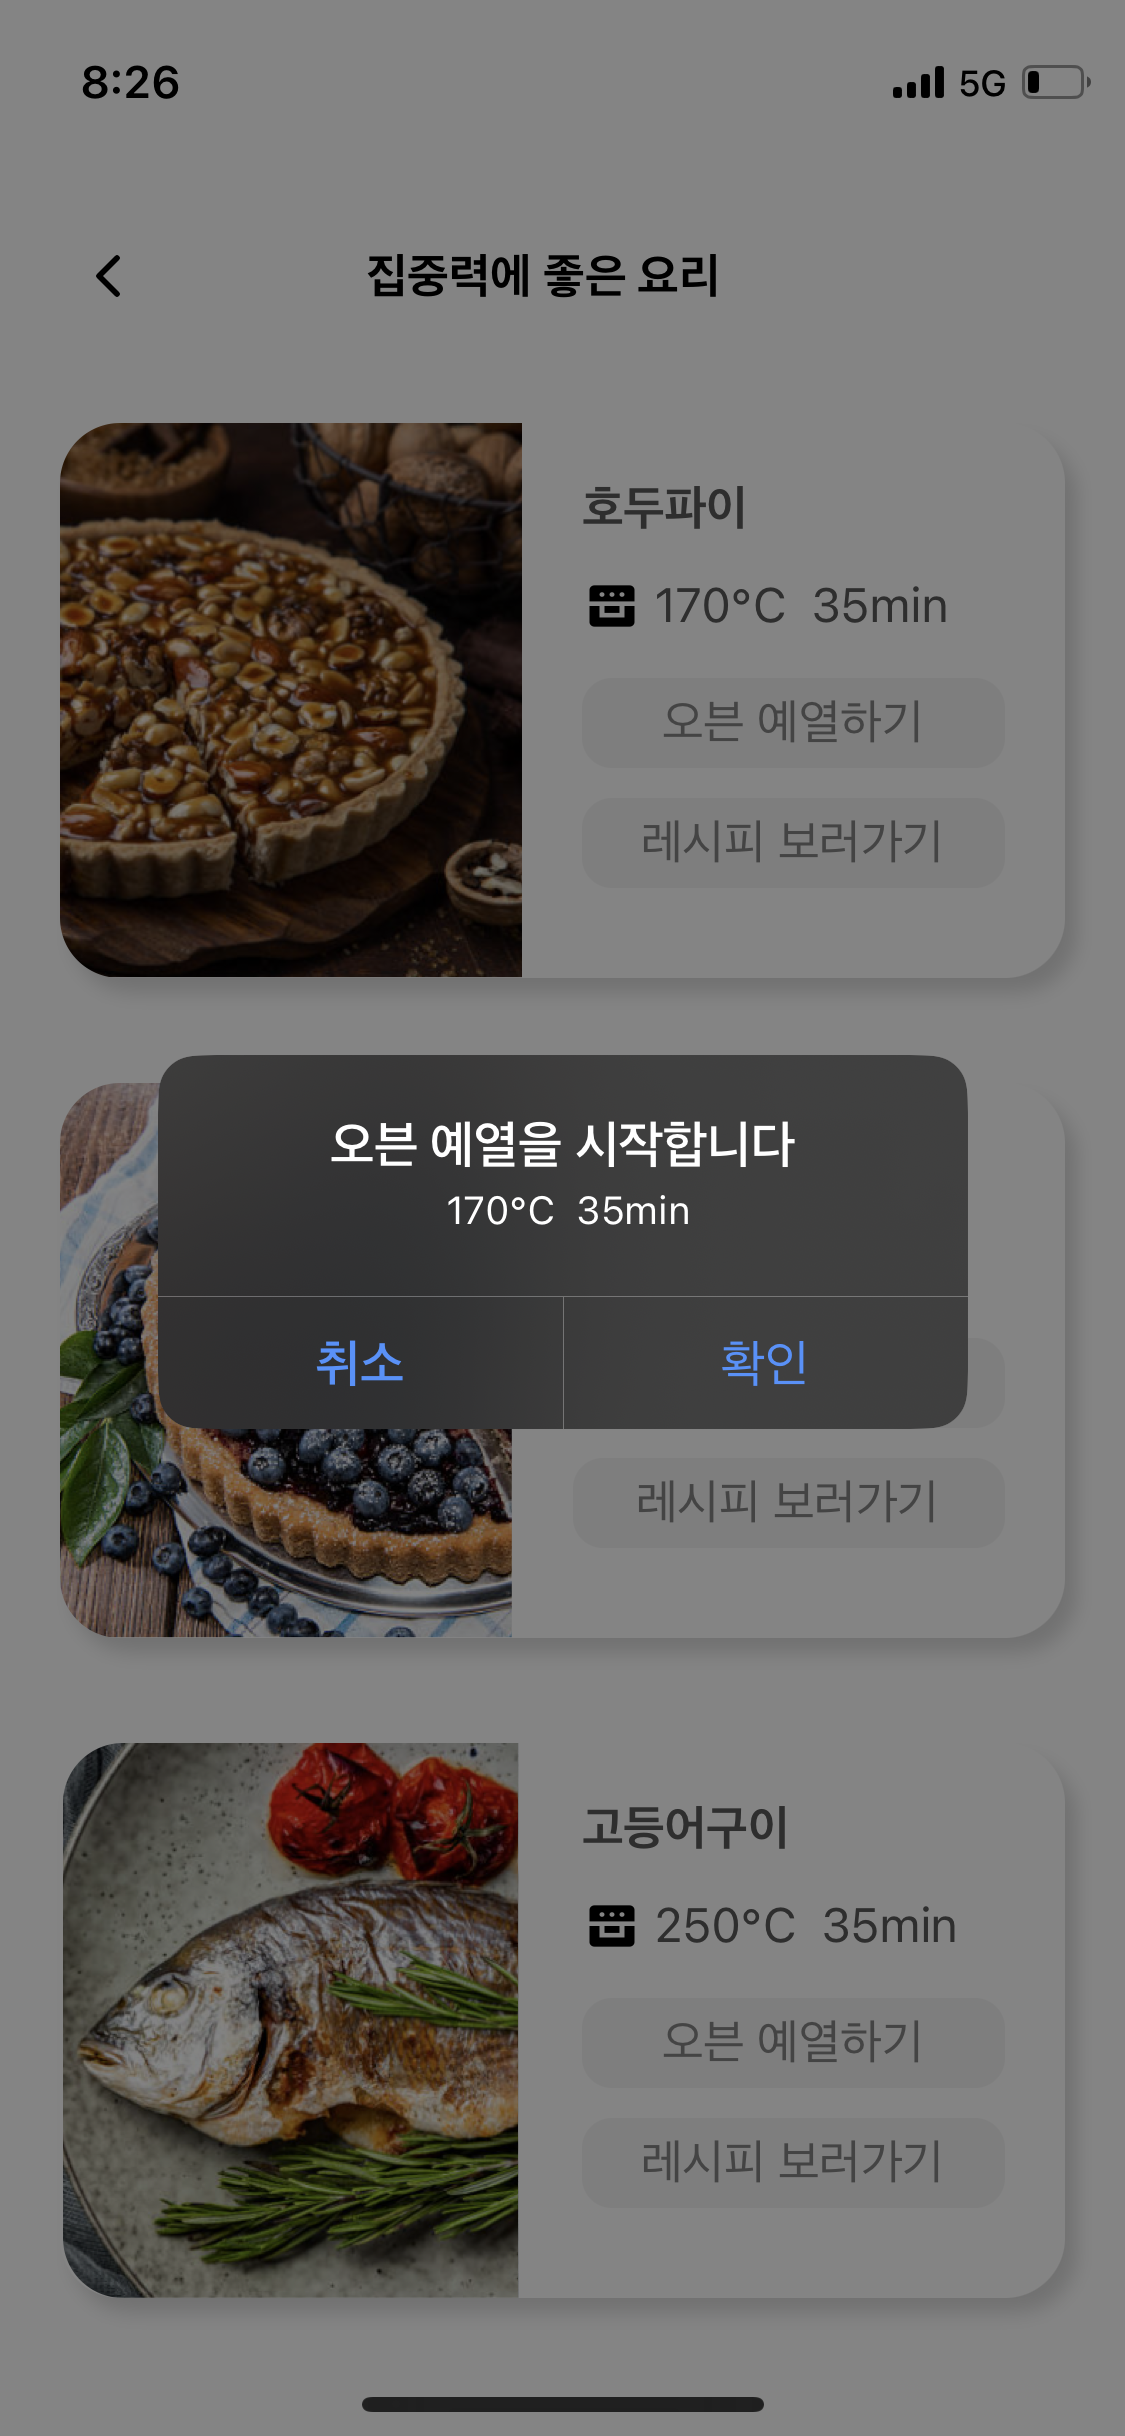
\includegraphics[scale=0.1]{s3.png}
                 \end{figure}
                \item AI speaker: Parent users can receive audiobook solutions through the interaction with AI speakers. In this case, user doesn't have to access the application. For example, when a user says, "Please play an audio book solution for my child's academic problem" to an AI speaker, it plays an audio book related to solution of child's academic problem.
                 \begin{figure}[H]
                 \centering
                 \includegraphics[scale=0.1]{sc4.png}
                 \end{figure}
            \end{enumerate}
\newpage
        \subsection{Child view}
        \begin{enumerate}
            \item Main page
            
            \begin{enumerate}
                \item When child-user successfully logged in, this page will firstly appear. In the today’s question section, which is shown to user first, child-user can look a question of parent. If there is no question arrived yet, icon and message appear at the page to inform user that there is no question. When there is a question registered, child-user can check it and go to answering page by clicking the button.
                \begin{figure}[H]
                 \centering
                 \includegraphics[scale=0.1]{ch1.png}
                 \includegraphics[scale=0.1]{ch2.png}
                 \end{figure}
                 
            \end{enumerate}
            \newpage
            \item Q\&A \hfill\break
            In this page, child-user can register his or her answer to the question. Child-user also can check today’s question above the input box for answering.
            \begin{figure}[H]
                 \centering
                 \includegraphics[scale=0.1]{a.png}
                 \includegraphics[scale=0.1]{a1.png}
                 \end{figure}
            \item Monthly child sentiment analysis page \hfill \break
            If child-user clicks the calendar icon, user can see monthly sentiment analysis result. This page looks like calendar, and each box of date shows face icon which indicates that day’s result of sentiment analysis as an expression. By clicking the box, user can check that day’s sentiment analysis result.
        \end{enumerate}
        \end{enumerate}
\newpage
\section{\large{Architecture Design \& Implementation}}
\subsection{Overall architecture}
\begin{figure}[H]
                 \centering
                 \includegraphics[scale=0.15]{diagram.png}
                 \end{figure}
                
Golden child consists of 5 modules: front-end, back-end, database, machine learning, AI speaker. The first module is the front-end. We used TypeScript languages and React Native, a cross-platform framework that supports both Android and IOS as mobile application frameworks. So all users can use our application regardless of their smartphone model. The reason why we used TypeScript language, not JavaScript, is that it is easy to identify errors when compiling and has high code readability. Our users are largely divided into two types: parent users and child users. Through the application, the parent user can ask the child one question every day. And the child user can register an answer to the question received by the parent through our application. When a child registers an answer, AI analyzes child’s feelings of the day. Then Our application provides the sentiment analysis result UI to parents and child users. Therefore, it allows parents to know about today's child's feelings conveniently. If the child's sentiment is negative, the parent may be provided with a solution that fits the child's current situation through the application.Second module is Backend. In our application, we use Django framework, which is based on the Python language as the web application server framework. The backend communicates with our application and AI speaker. Especially, The back-end server communicates with the front-end and AI speakers through the REST API. And we used Google Cloud Platform for server deployment.
Third  module is database. We used django’s basic SQlite for database. SQLite is basic option for Python, and it is to use SQLite for Django settings. We stored user information, question from parents, answer from children, and sentiment analysis in SQLite. Fourth module is machine learning. In machine learning part, We used KoBERT model. KoBERT is a Korean version of the BERT model. We used KoBERT to create a model that categorizes Korean sentences into seven emotions: joy, sadness, anger, hurt, embarrassment, anxiety. In our application, if the child leaves the answer, This answer goes into the input value of the KoBERT model we made, and as the output value, the results of six sentimental analysis according to the KoBERT model come out. This allows the parent user to see the percentage value based on each sentiment. Last module is AI speaker. We used AI speaker to interact with user. Parent user can receive the results of their child's sentiment analysis through AI speaker, listen to audiobook solutions related to their children's sentiment, and use some services related to home appliances. Voice interactions with AI speaker are developed in developer website.

\subsection{Directory Organization}
\begin{enumerate}
    \item front-end
    \begin{flushleft}
        \tablefirsthead{\toprule Directory & File name & etc \\ \midrule}
        \tablehead{\toprule Directory & File name & etc\\ \midrule}
        \tabletail{\midrule }
        \tablelasttail{\bottomrule}
        \begin{supertabular}{p{0.5\linewidth} | p{0.3\linewidth} p{0.05\linewidth}}
        /frontend/aurum & \makecell[l]{app.json\\App.tsx\\babel.config.js\\declaration.d.ts\\metro.config.js\\package.json\\tsconfiig.json\\yarn.lock\\.gitignore}\\
        \midrule
        /frontend/aurum/assets & \makecell[l]{splash.png\\icon.png\\favicon.png}\\
        \midrule
        /frontend/aurum/assets/fonts & \makecell[l]{Poppins-Black.ttf\\Poppins-Bold.ttf\\Poppins-Regular.ttf\\Poppins-Thin.ttf}\\
        \midrule
        /frontend/aurum/assets/icons & \makecell[l]{Babychick.svg\\Chicken.svg\\calendar.svg\\leaves.svg\\loveletter.svg\\studycgild.svg\\oven.svg\\TV.svg}\\
        \midrule
        \makecell[l]{/frontend/aurum/assets/icons\\/ChildIcons} & \makecell[l]{ChildAngry.svg\\ChildDefault.svg\\ChildHappiness.svg\\ChildSad.svg}\\
        \midrule
        \makecell[l]{/frontend/aurum/assets/icons\\/Sentiment} & \makecell[l]{anger.svg\\anxiety.svg\\default.svg\\embarrassment.svg\\happiness.svg\\injury.svg\\sadness.svg}\\
        \midrule
        \makecell[l]{/frontend/aurum/src} & \makecell[l]{index.tsx\\indexChild.tsx}\\
        \midrule
        \makecell[l]{/frontend/aurum/src/\\components} & \makecell[l]{DateDisplay.tsx\\Divider.tsx\\Header.tsx\\Logo.tsx\\MainCard.tsx\\NotificationBell.tsx\\PrimaryButton.tsx\\SentimentalAnalysis\\ReslutDisplay.tsx}\\
        \midrule
        \makecell[l]{/frontend/aurum/src/\\interfaces} & \makecell[l]{text.ts}\\
        \midrule
        \makecell[l]{/frontend/aurum/src/\\pages/Admin} & \makecell[l]{category.tsx\\info.tsx}\\
        \midrule
        \makecell[l]{/frontend/aurum/src/\\pages/Answer} & \makecell[l]{AnswerDisplay.tsx\\index.tsx\\QuestionDisplay.tsx}\\
        \midrule
        \makecell[l]{/frontend/aurum/src/\\pages/Login} & \makecell[l]{index.tsx}\\
        \midrule
        \makecell[l]{/frontend/aurum/src/\\pages/MonthlyView} & \makecell[l]{Calendar.tsx\\index.tsx\\MonthDisplay.tsx}\\
        \midrule
        \makecell[l]{/frontend/aurum/src/\\pages/Question} & \makecell[l]{AnswerDisplay.tsx\\index.tsx\\QuestionDisplay.tsx\\YesterdayDisplay.tsx}\\
        \midrule
        \makecell[l]{/frontend/aurum/src/\\pages/Solution} & \makecell[l]{Header.tsx\\indexStudy.tsx\\recipe.tsx\\RecipeDetail.tsx\\SolutionCard.tsx\\Speaker.tsx\\TodaySolution.tsx}\\
        \midrule
        \makecell[l]{/frontend/aurum/src/\\pages/SolutionCategories} & \makecell[l]{index.tsx}\\
        \midrule
        \makecell[l]{/frontend/aurum/src/utils} & \makecell[l]{const.ts\\fetchWithAuthentication.ts\\getAnswer.ts\\getLatestQuestion.ts\\getQuestion.ts\\getQuestions.ts\\getRepresentEmotion.ts\\getTodayInString.ts\\isLogin.ts\\loginWithCredentials.ts\\uploadQuestion.ts\\uploadAnswer.ts}\\
        \end{supertabular}
    \end{flushleft}
    \item back-end
    \begin{flushleft}
        \tablefirsthead{\toprule Directory & File name & etc \\ \midrule}
        \tablehead{\toprule Directory & File name & etc\\ \midrule}
        \tabletail{\midrule }
        \tablelasttail{\bottomrule}
        \begin{supertabular}{p{0.5\linewidth} | p{0.3\linewidth} p{0.05\linewidth}}
        /backend/golden\_child & \makecell[l]{manage.py}\\
        \midrule
        /backend/golden\_child/texts & \makecell[l]{\_\_init\_\_.py\\admin.py\\apps.py\\models.py\\serializers.py\\tests.py\\urls.py\\views.py}\\
        \midrule
        /backend/golden\_child/users & \makecell[l]{\_\_init\_\_.py\\adapters.py\\admin.py\\apps.py\\models.py\\serializers.py\\tests.py\\urls.py\\views.py}\\
        \midrule
        \makecell[l]{/backend/golden\_child/\\golden\_child} & \makecell[l]{\_\_init\_\_.py\\asgi.py\\settings.py\\urls.py\\wsgi.py}\\
        \end{supertabular}
    \end{flushleft}
    \item ai
    \begin{flushleft}
    \tablefirsthead{\toprule Directory & File name & etc \\ \midrule}
        \tablehead{\toprule Directory & File name & etc\\ \midrule}
        \tabletail{\midrule }
        \tablelasttail{\bottomrule}
        \begin{supertabular}{p{0.5\linewidth} | p{0.3\linewidth} p{0.05\linewidth}}
        ai/ & \makecell[l]{\_\_pycache\_\_\\.gitattributes\\.gitignore\\KoBERT\_model.pt\\README.md\\\_\_init\_\_.py\\common.py\\inference.py\\requirements.txt\\training.py}\\
        \end{supertabular}   
    \end{flushleft}
\end{enumerate}
\newpage
\subsection{Module}
\begin{enumerate}
    \item Front-end
       \begin{enumerate}
           \item Purpose
           \\It is used to provide users with records of Question \& Answer contents. It is also used to provide sentimental analysis result according to child answer and guide parents user how to behave. Therefore it is to receive user information and care their child with affection.
           
           \item Functionality
           \\First of all, it provides a registration function that distinguishes two types of users. If User logs in after signing up as a member, the functions user can receive vary depending on their type. If User type is a parent, it provides with functions such as registering today's questions, checking the child's answers, receiving child sentiment analyze result, and comparing the changes from yesterday's sentiment. In addition, it also provides functions of receiving parenting coaching according to child sentiments and recommending home appliance services suitable for coaching respectively. If User type is a child, It provides with functions such as registering today's answer, confirming parent's question, and receiving their sentiment analysis result.

           \item Location of Source Code
           \\/frontend/aurum

           \item Class Component
           \begin{enumerate}
               \item Sign Up page
               \\Since we need to receive a lot of information from users over multiple pages when signing up, we manage multiple components within one file. In this file, it is easy to manage user information such as user's email, password, and name. The most important information that this should receive is the user's type variable, which is managed by another file. Therefore, when the user signs up for a membership, the user first selects the user type, whether it is a parent or a child, and then inputs his/her information. If the type is not selected, it is impossible to sign up as a member by not moving to the information input page. For this, We use useState function in React Native, to manage the value that changes in the component.
               \item Sign In page
               \\This is the default routing page of the bottom tab bar. Therefore, We use React Navigation Library, Page navigation was implemented. There is an inputText that receives an ID, password and a lot of user information. However The ID and password are only managed within fetchwithAuthentication function file. This function performs the function of user authentication by checking whether the user has a token. And this function is always used when connecting to a server to retrieve questions or answers. When User clicks the login button, put the ID and password in the request body and send server uses the Axios library and is processed asynchronously. In this case, React hooks are used.
               \item Main Page \_ User Type : Parents
               \\On this page, parents can check their child's current status. This state is received through communication with the server when this page is first rendered. First, the date of the day is taken through the Date default function. Next, it is possible to check whether the child has registered the answer today or has not yet registered. If the answer is registered, the child icon on the main screen changes depending on the child's emotional analysis result on the server. All sentimental child icons are imported from the assets folder. To manage this variable value and handle asynchronous tasks, we used useEffect and useState functions. In addition, there is a calendar button on the main page that allows parents to check their children's monthly emotions as a whole. This monthly emotion also brings the response of the child on the server, sets the representative emotion based on the emotion analysis result. If the parent has not yet filled out the today question, an expressionless child icon will be visible in which case the parent can use the "Fill out the question" button at the bottom to go to the next page. This movement used the Stack Navigation Library of React Native.
               \item Question Page
               \\If the parent user has not yet registered the question, click the Register Question button on the main page to move to this page. Here, parents can register questions, and if the child has registered an answer, they can check it. React hooks are used to process asynchronous actions for parent's question registration process. The buttons and Displaying Today Date in the component are imported from the common folder. When a parent registers a question, the alert function is used to ask if they really want to send this question to the child. If the parent presses the confirmation button here, the parent question is posted to the server.
               \item Sentimental Analysis Result Display Page
               \\These components is that both parents and children can be seen if they register for question and answer, respectively. The results of Child emotion analysis are received from the server. And We calculate the emotion with the highest percentage of the results received today. For this process, six emotions that can be calculated in the AI library are put into one array and sorted. When the top three emotions are calculated in that way, only these emotions are shown to parents and children as a result. In addition, the progress bar library was used in this process to allow users to more explicitly check the child's emotional percentage. Every emotion icon has been imported from the asset folder. This process was asynchronously performed through the react hook. In addition to this component, it would be convenient for users to compare it with yesterday's emotion. Therefore, yesterday's result also calculated in the same way as received from the server, and then showed the result to the user. This component exists separately from today's emotion analysis result component.
               \item Solution Categories Page
               \\This page allows parents to choose whether to move or not depending on the child's current state. If the child's emotions are negative and parents want to receive parenting coaching, they can go to this page to check the solution. The content of the button changes depending on the child's representative feelings today. This button is a component that can be clicked on the emotion analysis result and answer confirmation page. There are five main categories of childcare, each managed as an ItemBox component. For example, if user clicks the study category, Study Drawer opens on the side. Parent users can find more detailed parenting coaching within the study category through this Drawer. Drawer was used as the Drawer Navigation library. Segmented coaching exists as a Screen in Drawer, and we have focused on the study category, especially among many coaching. Several solution components were imported for a movable Screen in Drawer.
               \item Solution Page
               \\This page is available when parents click on subdivided parenting coaching on Drawer in the solution category page. It is a page containing solution information that can solve the child's current state. Here, if parents want to hear the child solution through an AI speaker rather than the text of the application, they can click the headphone button in the header component. If user wants to listen to it on a speaker later, not right now, user can designate the current solution page as ‘Today's Solution’. Both go through the process of asking the user one more time through the alert function. If the user nevertheless presses the confirmation button in alert function, the current page is posted to the server as ‘Today's Solution’. This headphone button and ‘Today's Solution' exist as separate components and should be imported from this page. Users can also be recommended to use appliances suitable for their solution here. This home appliance recommendation also exists through Solution Card component. This recommendation varies from solution to solution. For example, if a child is anxious due to poor concentration, the user is recommended to operate an oven that prepares some food that increases concentration. In this case, If the user clicks on the Oven Solution Card component, user can move to the appropriate oven page.
               \item Main Page \_ User Type : Child
               \\From this page, child user can check whether the parent has registered a question or not. If a question is registered, child user can also check the contents of the question. This state is received through communication with the server when this page is first rendered. Also, if the user type is a child, this is the first root page to be displayed. First, the date is displayed with the date default function just like the parent's main page. Child user can check the parent's question registration status, and in each case, the icons they can see is different. When the question is registered, the love letter icon is displayed. all sub icons are imported from the assets folder. The useEffect and useState functions were used to manage this variable value and handle asynchronous operations. In addition, there is a calendar button on the main page, so child user can check their monthly emotions as a whole. This monthly emotion also received from the server and established representative emotions based on the results of the child sentimental analysis. Child user can go to the next page using the "Create Answer" button at the bottom. This movement used a React native stack navigation library.
               \item Answer Page
               \\If child user has not already registered an answer, click the Register Answer button on the main page to move this page. Here, the child user may check the parent's question and register an answer corresponding it. React Hook is used to handle asynchronous actions for the child's answer registration process. The buttons on the components and today's date display are imported from a common folder. Once the child user has registered for an answer, use the alert function to ask if they really want to send this answer to their parents. If the child user presses the confirmation button here, their answer will be posted to the server.
               
           \end{enumerate}
           \item Where it’s taken from
           \\Both child and parent users input their data, and previous data is retrieved from database.
           
           \item How/Why we used the module
           \\React-Native is a cross-platform framework that supports both Android and IOS as mobile application frameworks. So all users can use our application regardless of their smartphone model. It also uses the target platform's standard rendering API, allowing applications to maintain fast performance.
           
       \end{enumerate}
    \item Back-end
        \begin{enumerate}
        \item Purpose
        \\In our application, User actions such as membership/login, generation of questions and answers, and storing emotional analysis results should be handled. Therefore, a backend server is needed. The reason why we chose django as our backend framework is that first, we can conveniently build API through the Django REST framework (DRF). In addition, We thought that it would be easy to build and manage the Artificial Intelligence model by using machine learning libraries such as pytorch in django backend server because django is also based on Python.
        
        \item Functionality
        \\Backend server provides REST APIs that respond to request from clients. When there are some requests for DB’s data, it properly responses with those requests.\\
        DRF provides TokenAuthentication. Through the TokenAuthentication, tokens are given for each user, and we can identify different users through these tokens. It is required for client-server setup.\\
        After we define the required model in the models.py file, the corresponding data is automatically generated in db.sqlite3 file. SQLite is provided by default in django. So it is automatically connected with django backend server.
        
        \item Location of Source Code
        \\/backend
        
        \item Class Component
        \begin{enumerate}
            \item texts/views.py
            \\In Django, views.py is responsible for sending a response to a request sent by the client. It has similar role of controller, which is in other general MVC Framework. In detail, view takes required data from the model. In our project, we used both APIView belonging to CBV and viewset belonging to helper class. texts/views.py has QuestionViewSet, AnswerViewSet, GetOneQuestionView, GetOneAnswerView, GetNUGUReply.
            \item users/views.py
            \\In Django, views.py is responsible for sending a response to a request sent by the client. It has similar role of controller, which is in other general MVC Framework. In detail, view takes required data from the model. In our project, we used both APIView belonging to CBV and viewset belonging to helper class. Users/views.py has UserViewSet and CurrentUserView. CurrentUserView provides the information of user who is currently logged in.

            \item texts/models.py
            \\Models.py is responsible for creating models in the django framework. When creating class-type data model in the models.py, django creates a data model in the database through object-relational-mapping (ORM). In texts/models.py, class Question has id, created\_at, user(id), and content fields. class Answer has id, created\_, user(id), question id, content, result\_happiness, result\_anxiety, result\_embarrassment, result\_sadness, result\_anger, result\_injury, result\_max\_sentiment fields.
            \item users/models.py
            \\Models.py is responsible for creating models in the django framework. When creating class-type data model in the models.py, django creates a data model in the database through object-relational-mapping (ORM). In users/models.py, class user has id, user\_type, email, linked\_user, created\_at, USERNAME\_FIELD fields.

            \item texts/serializers.py
            \\Serializer serves as an adapter that converts complex objects such as queryset and model instances that we use in Django into json-like forms that we will use in the REST API. Today's API servers typically use JSON encoded requests/responses. texts/serializers.py has three serializers. QuestionSerializer, AnswerSerializer and SentimentSerializer.
            \item users/serializers.py
            \\Serializer serves as an adapter that converts complex objects such as queryset and model instances that we use in Django into json-like forms that we will use in the REST API. Today's API servers typically use JSON encoded requests/responses. users/serializers.py has two serializers. UserSerializer and CustomRegisterSerializer. dj\_rest\_auth basically uses RegisterSerializer when signing up for membership. We created a CustomSerializer that inherits the Register Serializer to receive additional custom fields.
            
            \item golden\_child/urls.py
            \\urls.py is a file that defines the URL address and the page to which the address should represent. In our project, golden\_child/urls.py contains all of urls in texts/urls.py and users/urls.py.  
            \item texts/urls.py
            \\urls.py is a file that defines the URL address and the page to which the address should represent. 'texts/single/question/' path requests one question. 'texts/single/answer/' path requests one answer. 'action.askSentiment' requests the result of sentiment analysis. 'action.hearAudiobook' requests audiobook play. 'action.askSentiment' and 'action.hearAudiobook' are related to the request of AI speaker.
            \item users/urls.py
            \\urls.py is a file that defines the URL address and the page to which the address should represent. 'users/user-list/' requests the list of all users. 'users/current-user/' requests the information of the currently logged-in user.
        \end{enumerate}
        \item Where it’s taken from
        \\Backend server takes data from our application and AI speaker.
        \item How/Why we use the module
        \\We used django because it is based on python language and it provides DRF(Django REST Framework), which is an open source library that is helpful for easily building a Restful API server within django.
        \end{enumerate}
    \item Database
        \begin{enumerate}
            \item Puropose
            \\We constructed database in order to manage the relationship of parent user and child user, including their question and answer. SQLite is table oriented relational database. In addition, it has the advantage of being easy to distribute with the app and move with the app as needed.
            
            \item Functionality
            \\Using SQLite, we set the relationships between data since SQLite is one of relational data systems. We set one-to-one relationship between parent-user and child-user. Answer and question also have relationship. Each question from parent can have only one answer from child. Also, the result of sentiment analysis is automatically saved in SQLite.
            
            \item Location of Source Code
            \\db.sqlite3
            
            \item Class Component
            \begin{enumerate}
                \item users\_user
                \\We can save and manage user information. It contains information such as the user type and e-mail received from the user when signing up. Also, if the user is child, parent's email value is also stored here.
                
                \item texts\_question
                \\It contains the questions left by the parents and the id value of the user who left the question. In addition, the date on which the question was created is automatically filled.
                
                \item texts\_answer
                \\The answer table contains the parent's question id value, the content of the child's answer to that question, and the user's id value who left the answer. And the information about the date when the answer was created is automatically generated, just like the question. Additionally, the results of the sentimental analysis of the child's answer are also stored in the answer table (ex - 80\% happiness, 10\% anxiety, etc.)       
            \end{enumerate}

            \item Where it’s taken from
            \\User information, questions, or answers are stored in the database through values entered by the user in the application.
            
            \item How/Why we use the module
            \\SQLite is built-in on Python, so we didn’t need to install it separately. Instead, by installing DB Browser for SQLite, We checked the table that we made.
            
        \end{enumerate}
        
    \item Machine learning
        \begin{enumerate}
            \item Purpose
            \\In our application, children leaves answer according to their parent’s question. By providing sentimental analysis results along with the child's response, parents can more efficiently grasp the child's response situation. In addition, in order to provide parents with a solution based on the child's emotion analysis results, we created an artificial intelligence model that analyzes the sentiments contained in Korean sentences using the KoBERT model. Parents can check how their child's sentiment have changed every day compared to the previous day, and they can understand at a glance the flow of child's overall sentiments from the calendar icon.
            
            \item Functionality
            \\When the child leaves an answer in the application, this answer goes into the input of the KoBERT model that we created. Six-sentiment (happiness, anxiety, embarrassment, sadness, anger, injury) analysis results for this input statement are then returned.
            
            \item Location of Source Code
            \\ai/
            
            \item Class Component
            \begin{enumerate}
                \item KoBERT\_model.pt
                \begin{figure}[H]
                 \centering
                 \includegraphics[scale=0.2]{BERT.png}
                 \end{figure}
                KoBERT is a Korean version of the BERT model, and it is pre-trained with a huge amount of data, so users can finetuning according to their purpose of use. KoBERT was developed to overcome the limitations of the existing BERT's Korean performance. It earned a large-scale corpus consisting of millions of Korean sentences collected by Wikipedia and News, and applied data-based tokenization techniques to reflect irregular language changes in Korean, resulting in a performance improvement of more than 2.6\% with 27\% tokens. By supporting various deep learning APIs, including PyTorch, TensorFlow, ONNX, and MXNet, it is contributing to the spread of language understanding services in many areas. After installing the necessary libraries and modules, we loaded the KoBERT file from GitHub. The KoBET model that we made is saved as KoBERT\_model.pt.
                \begin{enumerate}
                     \item Tain\_test\_split
                \\Using the train\_test\_split library provided by SKlearn, the dataset was divided into train data for model learning and test data for model evaluation. The ratio is 4:1.
                \item BERTSentenceTransform
                \\After dividing the dataset into train data and test data, we performed tokenization, integer encoding, and padding so that each data could enter the input of the KoBERT model. Tokenization and padding are done through the BERTSentenceTransform module.
                \item BERTClassifier
                \\We created a KoBERT model for learning through the BERTClassifier. We specified the num\_classes variable as many classes as we wanted to multi-classify. In our project, we classified 6 sentiments, so we entered num\_classes as 6.
                \end{enumerate}
                \item common.py \\
                In common.py, After the data is preprocessed, the setting for model learning is started. Artificial Intelligence model will be learned according to the setting parameters set here.
                \item training.py\\
                Once the model is learned, we must save the entire model that is learned. We wrote code to store the model in training.py.
                \item inference.py\\
                After saving the model, we recall and use the learned model in inference.py. 
            \end{enumerate}
            
            \item Where it’s taken from
            \\The answer that the child user left in the application becomes the input value of the KoBERT model. Then model returns the values of 6 sentiment, as the result of sentiment analysis.
            
            \item How/Why we use the module
            \begin{enumerate}
                \item PyTorch
                \\Torch is an open source machine learning library. After PyTorch model is saved, it is loaded into our application. 
                \item Pandas
                \\Pandas is a software library used in Python, which is for data manipulation and analysis. We used pandas in the process of reading the dataset and preprocessing the data to suit our purpose.
                \item Numpy
                \\Numpy is Python's library that facilitates the processing of multidimensional arrays. It also provides an efficiently implemented function for numerical computation.
            \end{enumerate}
        \end{enumerate}
        
    \item AI speaker
        \begin{enumerate}
            \item Purpose
            \\Using AI Speaker makes it more convenient for parents who have been busy and have not had time to look into the application, or want to conveniently grasp their children's sentiments and receive related solutions while spending their personal time.
            
            \item Functionality
            \\ Parents can conveniently check the child's sentimental analysis results and receive solutions related to their child's sentiment through interaction with AI speakers at home.
            \begin{figure}[H]
            \centering
            \includegraphics[scale=0.3]{new_assets/nugu-play-1.png}
            \end{figure}
            
            \item Location of Source Code
            \\AI Speaker Play Builder
            
            \item Class Component
            \begin{enumerate}
                \item intent.askSentiment
                \\When the user says, "Tell me the result of the child's sentimental analysis today," the speaker takes the sentimental analysis results from the back-end server and returns them to the user. The entity is set for the date, so the speaker automatically recognizes and distinguishes the dates such as 'yesterday', 'today', and 'tomorrow'.
                \begin{figure}[H]
            \centering
            \includegraphics[scale=0.5]{new_assets/nugu-play-sentiment.png}
            \end{figure}
                
                \item intent.hearAudiobook
                \\When the user says, "Play today's audiobook solution", the speaker plays the corresponding audiobook solution. In the example sentence above, the audiobook solution becomes entity.
                
                \item intent.heatOven
                \\The parent user can preheat the oven under desired conditions through the speaker. For example, if a parent wants to preheat the oven to 170 degrees when cooking for a child, it is possible to preheat the oven through the utterance "Preheat the oven to 170 degrees.”
                \begin{figure}[H]
            \centering
            \includegraphics[scale=0.5]{new_assets/nugu-play-oven.png}
            \end{figure}
                
                \item intent.setAlarm
                \\Parent users can set alarms to automatically play child sentiment analysis results on AI speaker at a specified time. For example, working parents can be set alarm to receive the child's sentimental analysis results at 10 p.m., the time after work.
                \begin{figure}[H]
            \centering
            \includegraphics[scale=0.5]{new_assets/nugu-play-alarm.png}
            \end{figure}
            \end{enumerate}
            
            \item Where it’s taken from
            \\AI speaker receive the data from user’s utterance.
            
            \item How/Why we use the module
            \begin{figure}[H]
            \centering
            \includegraphics[scale=0.5]{new_assets/nugu_intent.png}
            \includegraphics[scale=0.5]{new_assets/nugu_action.png}
            \end{figure}
            The speaker returns the information that the user wants to obtain through the user's speech. Users can receive today's solution based on their child's sentimental analysis through the speakers. In addition, the oven is interlocked through interaction with the speaker, allowing the user to set the oven preheating setting as desired.
            
        \end{enumerate}
\end{enumerate}
\clearpage
\section{\large{Use Cases}}
\subsection{Mobile Application}
\begin{figure}[H]
\centering
\includegraphics[scale=0.1]{signup.png}
\end{figure}
When person who use Golden Child for the first time, login page will be shown at first. If login is successful, it goes to the main page depending on the user type.
\begin{enumerate}
    \item Parent User
    \begin{enumerate}
        \begin{figure}[H]
        \centering
        \includegraphics[scale=0.1]{signup2.png}
        \includegraphics[scale=0.1]{signup3.png}
        \end{figure}
        \item Use Case 1 
        \\The user who downloaded this application inputs member information to complete the sign up process. In particular, a user type must be selected whether it is a child user or a parent user. And then the visible main page is changed accordingly. If user type is not selected, sign up process is not possible.
        \begin{figure}[H]
        \centering
        \includegraphics[scale=0.1]{main1.png}
        \includegraphics[scale=0.1]{main.png}
        \includegraphics[scale=0.1]{main2.png}
        \includegraphics[scale=0.1]{main3.png}
        \end{figure}
        \item Use Case 2
        \\On the main page, if Parent user have not already registered a question to the child, they will be asked to enter the question. And Parent user can see an expressionless child icon in the main page. If parent user register the question, the expression of the child icon changes according to the child's current feelings.
        \begin{figure}[H]
         \centering
         \includegraphics[scale=0.1]{mon2.png}
         \includegraphics[scale=0.1]{mon1.png}
         \end{figure}
        \item Use Case 3
        \\Parent user can check the monthly sentimental analysis report by clicking the calendar icon on the main page. On the calendar, icons reflecting the emotions of the child day by day are displayed. This emotion is set as the representative emotion with the highest percentage of the child's emotion analysis results on the day.
        \begin{figure}[H]
        \centering
        \includegraphics[scale=0.1]{q.png}
        \includegraphics[scale=0.1]{q1.png}
        \includegraphics[scale=0.1]{q2.png}
        \end{figure}
        \item Use Case 4
        \\If the parent user has not yet registered the question, click the Register Question button on the main page. When a parent completes the registration of a question, it goes through the alert window to confirm whether they really want to register the question.
        \begin{figure}[H]
        \centering
        \includegraphics[scale=0.1]{qa1.png}
        \end{figure}
        \item Use Case 5
        \\If the child user leaves an answer according to the question left by the parent, the sentimental analysis result of this answer is automatically displayed. Also, at the bottom of the screen, parent user can compare yesterday's child's feelings with today's feelings
        \begin{figure}[H]
        \centering
        \includegraphics[scale=0.1]{sc.png}
        \includegraphics[scale=0.1]{sc1.png}
        \includegraphics[scale=0.1]{sc3.png}
        \end{figure}
        \item Use Case 6
        \\If the child's emotions are negative and parenting coaching is needed for the answer, the parent user goes to the solution page by clicking the solution button. The content of this button changes according to the child's feelings. When parent users go to the solution page, they can first select the child's solution category and select contents of the specific audio book.
        \begin{figure}[H]
        \centering
        \includegraphics[scale=0.1]{s.png}
        \includegraphics[scale=0.1]{s1.png}
        \includegraphics[scale=0.1]{s3.png}
        \includegraphics[scale=0.1]{s2.png}
        \includegraphics[scale=0.1]{s4.png}
        \end{figure}
        \item Use Case 7
        \\After the parent user checks the contents of the solution that fits the child's situation, there is a customized home appliance service tab at the bottom of the page. For example, if parent users select the study-related solution category, they can use the TV viewing restriction function to create a child's learning environment, and oven preheating function to make foods that enhance child’s concentration. The parent users may also browse the recipe for cooking the food. If they want to listen to this solution on their speaker right now, they can click on the headphone button in the header. If they want to listen later, click the 'Today’s Solution' button. Then, this solution becomes the 'Today’s solution', and the parent user can listen to this at any time through the AI speaker.
        \begin{figure}[H]
        \centering
        \includegraphics[scale=0.1]{sc2.png}
        \includegraphics[scale=0.1]{sc4.png}
        \end{figure}
    \end{enumerate}
    \newpage
    \item Child User
    \begin{enumerate}
        \begin{figure}[H]
        \centering
        \includegraphics[scale=0.1]{ch1.png}
        \includegraphics[scale=0.1]{ch2.png}
        \end{figure}
        \item Use Case 1 
        \\If question has not yet registered from the parent user, the main page displays the phrase "The question has not arrived yet." Also, the leaves icon, not the love letter icon, is displayed. If a parent user registers a question, the love letter icon is displayed, and the contents of the parent's question can be shown. If child user want to register an answer that corresponds to the parent’s question, click the button at the bottom to move the page where child user can write an answer.
        \begin{figure}[H]
         \centering
         \includegraphics[scale=0.1]{mon2.png}
         \includegraphics[scale=0.1]{mon1.png}
         \end{figure}
        \item Use Case 2
        \\Child user can check the monthly emotion analysis report by clicking the calendar icon on the main page. The calendar is marked with icons that reflect one's feelings day by day. This emotion is set as a representative emotion with the highest percentage of one's emotion analysis results on the day. This screen looks the same as when the user type is a parent.
        \begin{figure}[H]
        \centering
        \includegraphics[scale=0.1]{a.png}
        \includegraphics[scale=0.1]{a1.png}
        \includegraphics[scale=0.1]{a2.png}
        \includegraphics[scale=0.1]{a3.png}
        \end{figure}
        \newpage
        \item Use Case 3
        \\When the child user completes the registration of the answer corresponding to the parent's question, it goes through the confirmation process through the alert window. Then, the emotion analysis result for the answer is automatically displayed in the application.
    \end{enumerate}
\end{enumerate}
\subsection{AI Speaker}
\begin{enumerate}
    \item Use Case 1 
    \\Parents who want to hear the results of child sentiment analysis through AI speaker would say "Tell me the results of child sentiment analysis”. Then the AI speaker would send a request to the database, receive the information from database, and then return the result of sentiment analysis to the user.
    \item Use Case 2
    \\The parent user can set an alarm to automatically play the child sentiment analysis result on the AI speaker at a specific time. Only when parents leave questions and children leave answers to them, parent can hear the results of the emotional analysis of the day. When this condition is satisfied, AI speaker would request and receive the sentiment analysis information from the database, and the child's sentiment analysis results are automatically played at a specific time set by the user.
    \item Use Case 3
    \\Parents who have heard the results of their children's emotional analysis can ask AI speakers to provide a "solution of the day" related to this. AI speakers play today's solution, which is saved as the form of audiobook solution. Today's solution can be directly designated as an audio book solution that users want among the contents in the application, and then later parent user can listen it conveniently at home through AI speakers.
    \item Use Case 4 
    \\Parents can use home appliance services related to their child's emotional analysis results through AI speakers. For example, if a parent wants to cook a concentration-enhancing dish for a child and the oven is required for that dish, the parent user can set the preheating of the oven to the desired condition (ex - 170 degrees), by using AI speaker conveniently.
\end{enumerate}
\newpage
\section{conclusion}
Golden Child can help parents and children communicate continuously even when they are away from each other in their busy daily lives. In addition, Golden Child provides parents with not only their child's answers to questions, but also their child's sentiment analysis results. We expect parents to understand their children better and communicate more smoothly with their children by receiving their child's sentimental analysis results and related audiobook/home appliance service solutions through Golden Child. \hfill\break \hfill\break
Future development of Golden Child
\hfill\break
\begin{enumerate}
    \item When parents and children leave questions and answers, they can use the app conveniently using the voice messaging function.
    \hfill\break
    \item Extend the home appliance service offered. (ex - refrigerator)
    \hfill\break
    \item Parents can get a holistic view of their child's day through the child's school and academy schedule management function.
    \hfill\break
    \item If the child's negative emotions persist for a certain period of time, it provides the ability to ask a specialist for counseling.
    \hfill\break
    \item Expand the scope of the audiobook solution category. Also, parents can see journals or articles related to childcare at a glance.
    \hfill\break
    \item We can introduce community for parents in Golden Child where parents communicate with each other about childcare and help each other. \hfill\break
    \hfill\break Golden Child's ultimate goal is that parents get to know their children better and  children build bonds with their parents.
\end{enumerate}

\clearpage
\begin{thebibliography}{00}

\bibitem{b1} Google Colab (https://colab.research.google.com/github/SKTBrain\\/KoBERT/blob/master/scripts/NSMC/\\naver\_review\_classifications\_pytorch\\\_kobert.ipynb\#scrollTo=itIExnuLbSap)
\bibitem{b2} SKT Brain KoBERT (https://github.com/SKTBrain/KoBERT)
\bibitem{b3} Fine-tuning Pre-trained BERT Models\\ (https://nlp.gluon.ai/examples/sentence\_embedding/bert.html)
\end{thebibliography}

    
\end{document}